% Use with CC terms.
% Adrin Jalali - 2013
%

\documentclass[final]{beamer} % beamer 3.10: do NOT use option hyperref={pdfpagelabels=false} !
%\documentclass[final,hyperref={pdfpagelabels=false}]{beamer} % beamer 3.07: get rid of beamer warnings
\mode<presentation> {  %% check http://www-i6.informatik.rwth-aachen.de/~dreuw/latexbeamerposter.php for examples
  %\usetheme{whale} 
  \usetheme{Berlin}  
}
\usepackage[english]{babel}
\usepackage[latin1]{inputenc}
\usepackage{amsmath,amsthm, amssymb, latexsym}
\usefonttheme[onlymath]{serif}
\boldmath
\usepackage[size=custom,width=95,height=130,scale=2,debug]{beamerposter}


\usepackage{beamerthemeshadow}
\usepackage[absolute,overlay]{textpos}
\usepackage{graphics}
\usepackage{colortbl}
\usepackage{xcolor}
\usepackage[absolute,overlay]{textpos}
\usepackage{sidecap}
\usepackage[labelformat=empty]{caption}
\usepackage{booktabs}

\setbeamercolor{framesource}{fg=gray}
\setbeamerfont{framesource}{size=\tiny}
\beamertemplatenavigationsymbolsempty

\newcommand{\source}[1]{\begin{textblock*}{4cm}(8.7cm,8.6cm)
    \begin{beamercolorbox}[ht=0.5cm,right]{framesource}
        \usebeamerfont{framesource}\usebeamercolor[fg]{framesource} {#1}
    \end{beamercolorbox}
\end{textblock*}}

\newcommand{\mycite}[1]{\begin{textblock*}{4cm}(8.7cm,8.6cm)
    \begin{beamercolorbox}[ht=0.5cm,right]{framesource}
        \usebeamerfont{framesource}\usebeamercolor[fg]{framesource} {#1}
    \end{beamercolorbox}
\end{textblock*}}


\newcommand{\mytitle}[1]{\large{#1} \hrulefill \\}

\definecolor{pathwaynode}{RGB}{255,150,50}
\definecolor{independentnode}{RGB}{255,255,50}
\newcommand{\boz}{\cellcolor{pathwaynode}}
\newcommand{\ghool}{\cellcolor{independentnode}}

\title[Gene Expression, PPI Network, Classification]{Analyzing How Protein Interaction Networks Improve Classification Performance in Gene Expression Data Analysis}
\author{Adrin Jalali and Nico Pfeifer}
\institute{Department of Computational Biology and Applied Algorithmics\\Max Planck Institute for Informatics\\Saarbr�cken, Germany}
%\date{\today} 
\date{}
%\titlegraphic{
\includegraphics[width=4cm]{mpi-logo}}
\begin{document}
\begin{frame}[plain]{}
  \maketitle
  \begin{textblock*}{\paperwidth}(0.1\textwidth,0.12\textheight)
    \raggedright
    
\includegraphics[width=0.2\textwidth]{mpi-logo}
  \end{textblock*}
  \begin{textblock*}{\paperwidth}(0.8\textwidth,0.11\textheight)
    \raggedright
    
\includegraphics[width=0.1\textwidth]{mpg-logo}
  \end{textblock*}

  \mytitle{Motivation}
  \begin{columns}
    \begin{column}{0.3\textwidth}
      \center
      \begin{figure}
        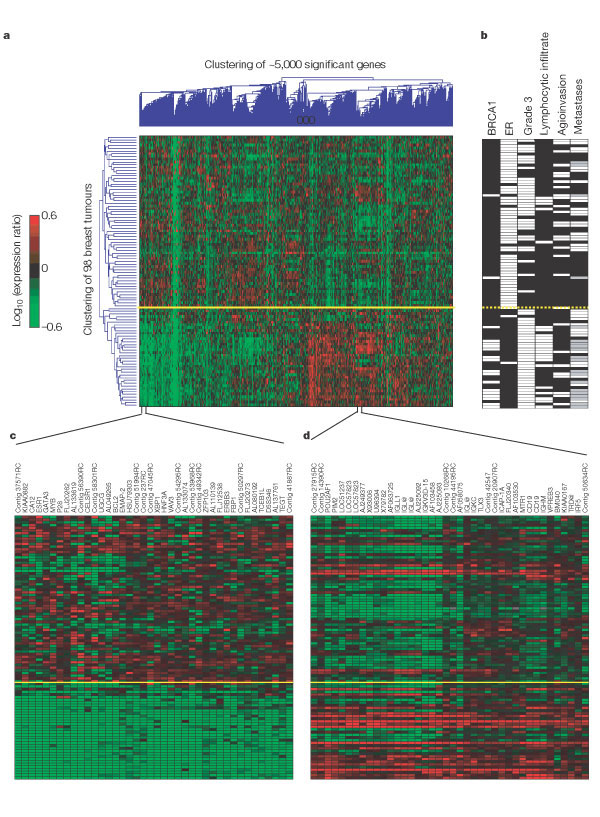
\includegraphics[height=20cm]{vantveer-summary}
        \caption{\tiny Unsupervised two-dimensional cluster analysis of 98 breast tumours [1]}
        \note{a, Two-dimensional presentation of transcript ratios for 98 breast tumours. There were 4,968 significant genes across the group. Each row represents a tumour and each column a single gene. As shown in the colour bar, red indicates upregulation, green downregulation, black no change, and grey no data available. The yellow line marks the subdivision into two dominant tumour clusters. b, Selected clinical data for the 98 patients in a: BRCA1 germline mutation carrier (or sporadic patient), ER expression, tumour grade 3 (versus grade 1 and 2), lymphocytic infiltrate, angioinvasion, and metastasis status. White indicates positive, black negative and grey denotes tumours derived from BRCA1 germline carriers who were excluded from the metastasis evaluation. The cluster below the yellow line consists of 36 tumours, of which 34 are ER negative (total 39 ER-negative) and 16 are carriers of the BRCA1 mutation (total 18). c, Enlarged portion from a containing a group of genes that co-regulate with the ER- gene (ESR1). Each gene is labelled by its gene name or accession number from GenBank. Contig ESTs ending with RC are reverse-complementary of the named contig EST. d, Enlarged portion from a containing a group of co-regulated genes that are the molecular reflection of extensive lymphocytic infiltrate, and comprise a set of genes expressed in T and B cells. (Gene annotation as in c.)}
        \note{http://www.nature.com/nature/journal/v415/n6871/full/415530a.html}
      \end{figure}
    \end{column}
    
    \begin{column}{0.3\textwidth}
        \footnotesize
        Problem statement:
      \begin{itemize}
          \item Input: Gene expression data
          \item Output: Prognosis (Poor vs. Good), Metastases
          \item Goal: Classify samples and find important genes
          \item Issue: Hard to classify due to large number of features (genes) compared to number of samples ($\sim 22000 \gg 98$)
      \end{itemize}
    \end{column}

    \begin{column}{0.3\textwidth}
      \begin{figure}
        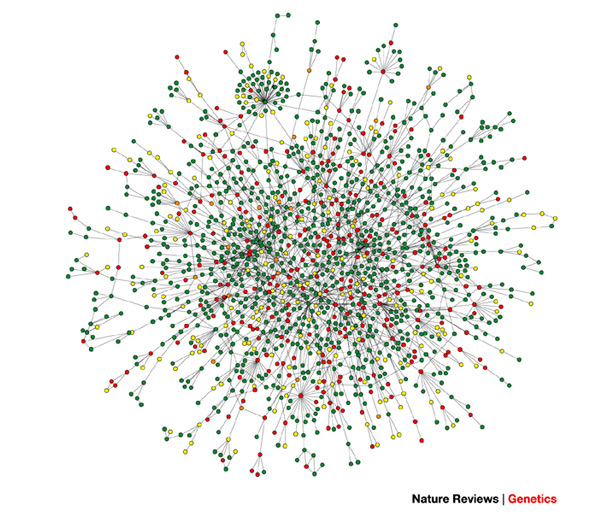
\includegraphics[width=0.8\textwidth]{yeastProteinInteractionNetwork}
        \caption{\tiny Yeast protein interaction network. The colour of a node indicates the phenotypic effect of removing the corresponding protein ({\color{red}red} = lethal, {\color{green}green} = non-lethal, {\color{orange}orange} = slow growth, {\color{yellow}yellow} = unknown) [2]}
      \end{figure}
      \note{http://www.nature.com/nrg/journal/v5/n2/fig_tab/nrg1272_F2.html}
    \end{column}
  \end{columns}

  \mytitle{Method}
    \begin{columns}
%      \begin{column}{0.25\textwidth}
%        %\frametitle{NICK Performance Summary}
%        \begin{figure}
%          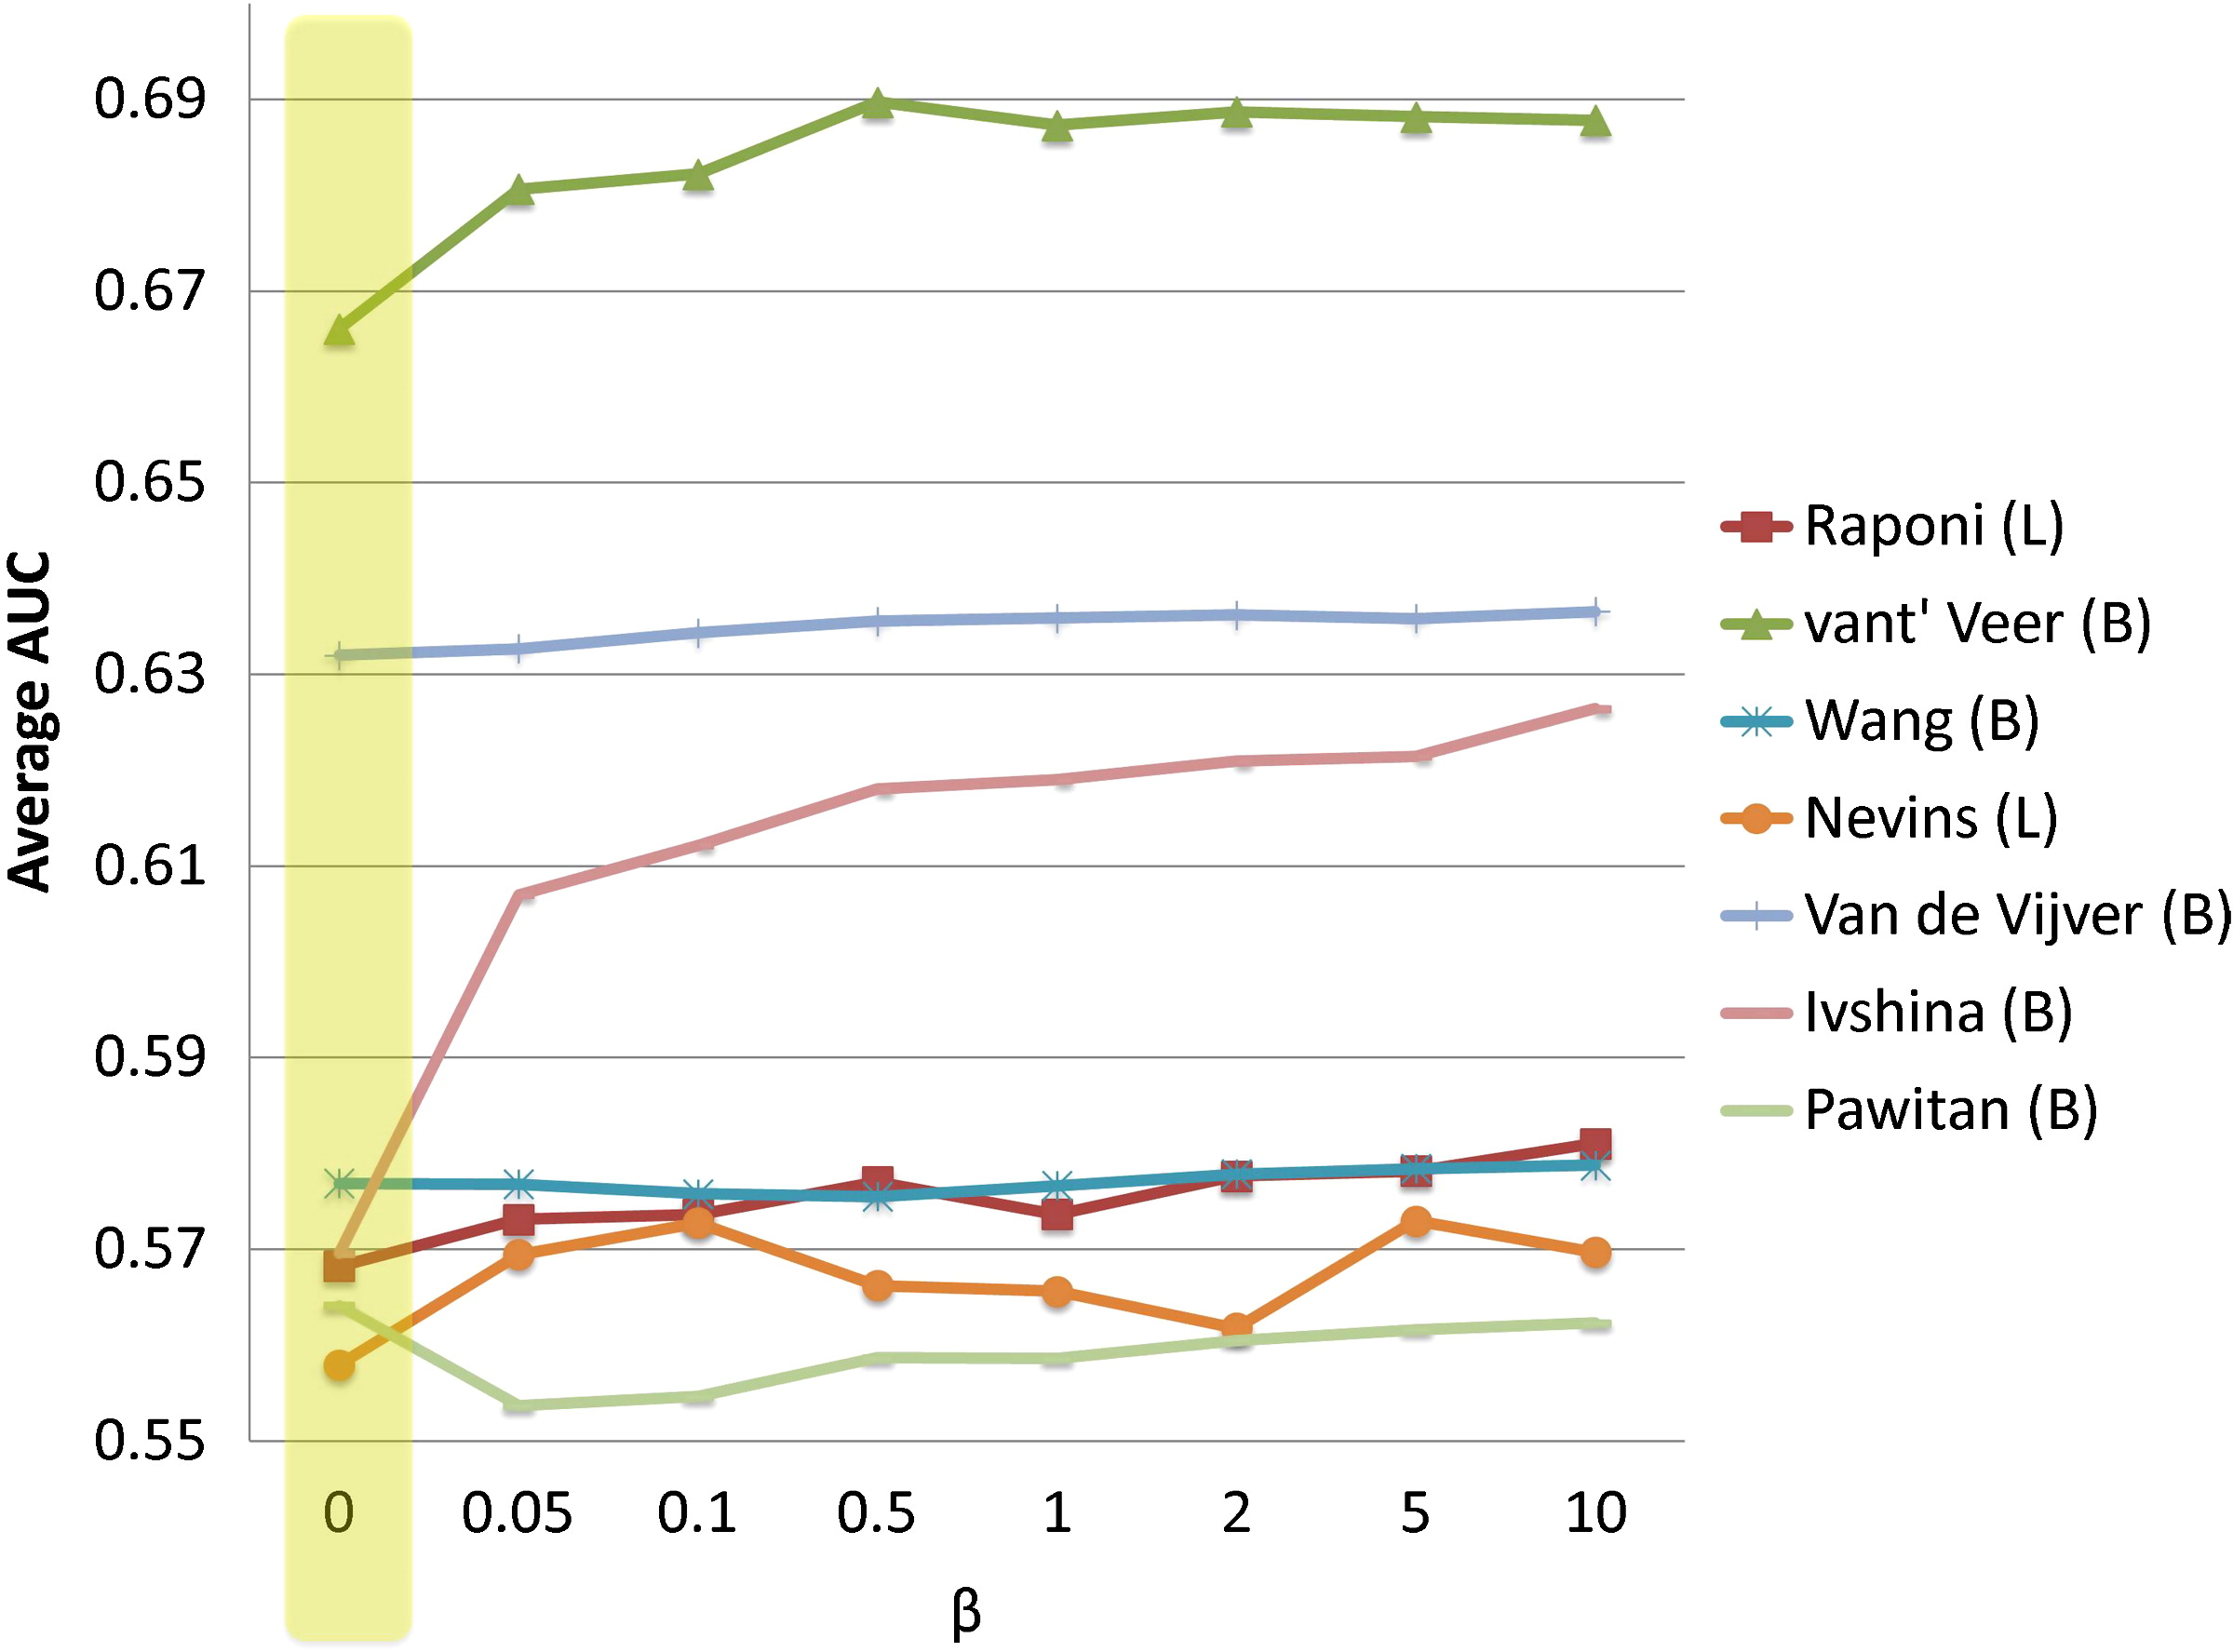
\includegraphics[width=0.9\textwidth]{NICK-perfs}
%          \caption{\tiny          1. Co-expressed genes tend to be close in the PPI-Network.
%            2. Exploit this fact to modify the SVM objective function - called NICK. Ofer Lavi, et.al., Journal of Computational Biology, (2012)
%          }
%        \end{figure}
%        %\mycite{Ofer Lavi, et.al., Journal of Computational Biology, (2012)}
%        \note{http://online.liebertpub.com/doi/full/10.1089/cmb.2012.0065}
%      \end{column}

      \begin{column}{0.3\textwidth}
        \vspace{1cm}
        \begin{enumerate}
          \footnotesize
        \item SVM modified objective function [3]
          \tiny
          \begin{center}
            \begin{align*}
              &\min_{\mathbf{w}, w_0}\left\{\frac{1}{2}\|\mathbf{w}\|^2 + \frac{1}{2}\beta\sum_{(j,k)\in E}(w_j-w_k)^2\right\}\\
              \text{s.t.:} &\\
              &\forall i \in \{1,\cdots,n\} : (\mathbf{w}\mathbf{x}_i+w_0)y_i\geq 1
            \end{align*}
          \end{center}
          
          \footnotesize
        \item Dual Problem
          \tiny
          \begin{center}
            \begin{align*}
              &\max_\alpha\left\{\sum_{i=1}^n\alpha_i-\frac{1}{2}\sum_{i=1}^n\sum_{j=1}^n\alpha_i\alpha_j y_i y_j (\mathbf{x}_i^T\mathbf{L})(\mathbf{L}^T\mathbf{x}_j)\right\}\\
              &\mathbf{L}\mathbf{L}^T=(\mathbf{I}+\beta \mathbf{B})^{-1}\\
              \text{s.t.: }&\\
              &\forall i \in \{1,\cdots,n\}: \sum_{i=1}^n\alpha_iy_i=0\\
              &\forall i \in \{1,\cdots,n\}: \alpha_i \geq 0 \\
              &\text{Laplacian matrix:}\\  & \mathbf{B} = \mathbf{D} - \mathbf{A}
            \end{align*}
          \end{center}

          \footnotesize
        \item Dual to Primal
          \tiny
          \begin{center}
            $\mathbf{w} = (\mathbf{I} + \beta \mathbf{B})^{-1} \sum_{i = 1}^n \alpha_i y_i \mathbf{x}_i$
          \end{center}
        \end{enumerate}
      \end{column}

      \begin{column}{0.3\textwidth}
          \footnotesize
        What we do:
        \begin{itemize}
          \item Reverse engineer the learned machine to extract important genes after using the network information.
          \item Solve SVM problem for original and transformed data.
          \item Calculate $\mathbf{w}$ for both models.
          \item Compute for each pair of nodes, for each model: 
              $Score(i, j) = \frac{|w_i| + |w_j|}{2} \times e^{-max\left(d_G(i, j), 1\right)}$
          \item Report pairs with highest scores for both trained models.
        \end{itemize}
      \end{column}
      %\mycite{Ofer Lavi, et.al., Journal of Computational Biology, (2012)}

      \begin{column}{0.3\textwidth}
        %\frametitle{Synthesize Data}
        \begin{figure}
          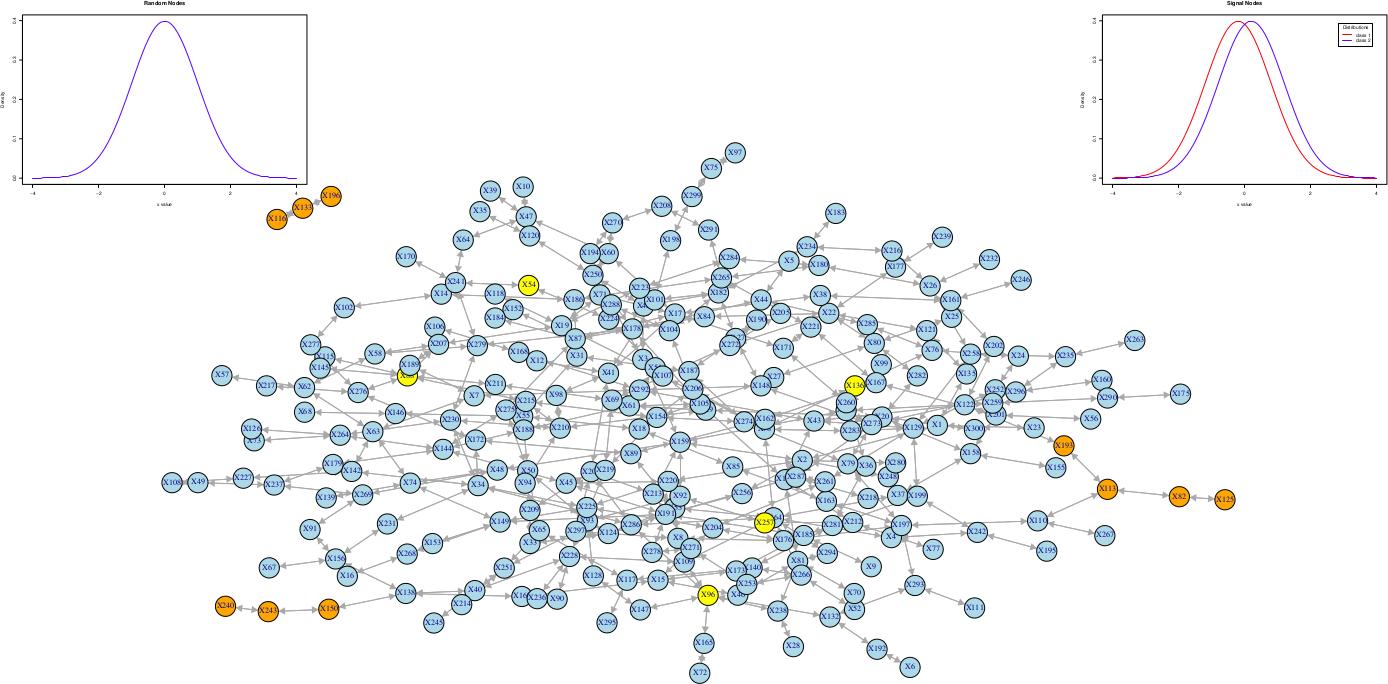
\includegraphics[width=0.8\textwidth]{synthesized-1slide}
          \caption{\tiny {\color{blue}Blue}: random gene, {\color{orange}Orange}: Signal node being a member of a pathway of signal nodes, {\color{yellow}Yellow}: A lonely signal node
        \\- Signal nodes (genes): $ f(n) = \left\{ 
          \begin{array}{l l}
            N(-\mu, 1) & \quad \text{if $n$ is in class $1$}\\
            N(\mu, 1) & \quad \text{if $n$ is in class $2$}
          \end{array} \right.$
        \\- Random nodes (non-informative genes): $f(n) = N(0, 1) $
          }
        \end{figure}
      \end{column}
    \end{columns}
  
  \mytitle{Results}
    \begin{columns}
      \begin{column}{0.3\textwidth}
        %\frametitle{Synthesized Data Easy Scenario}
        \begin{figure}
          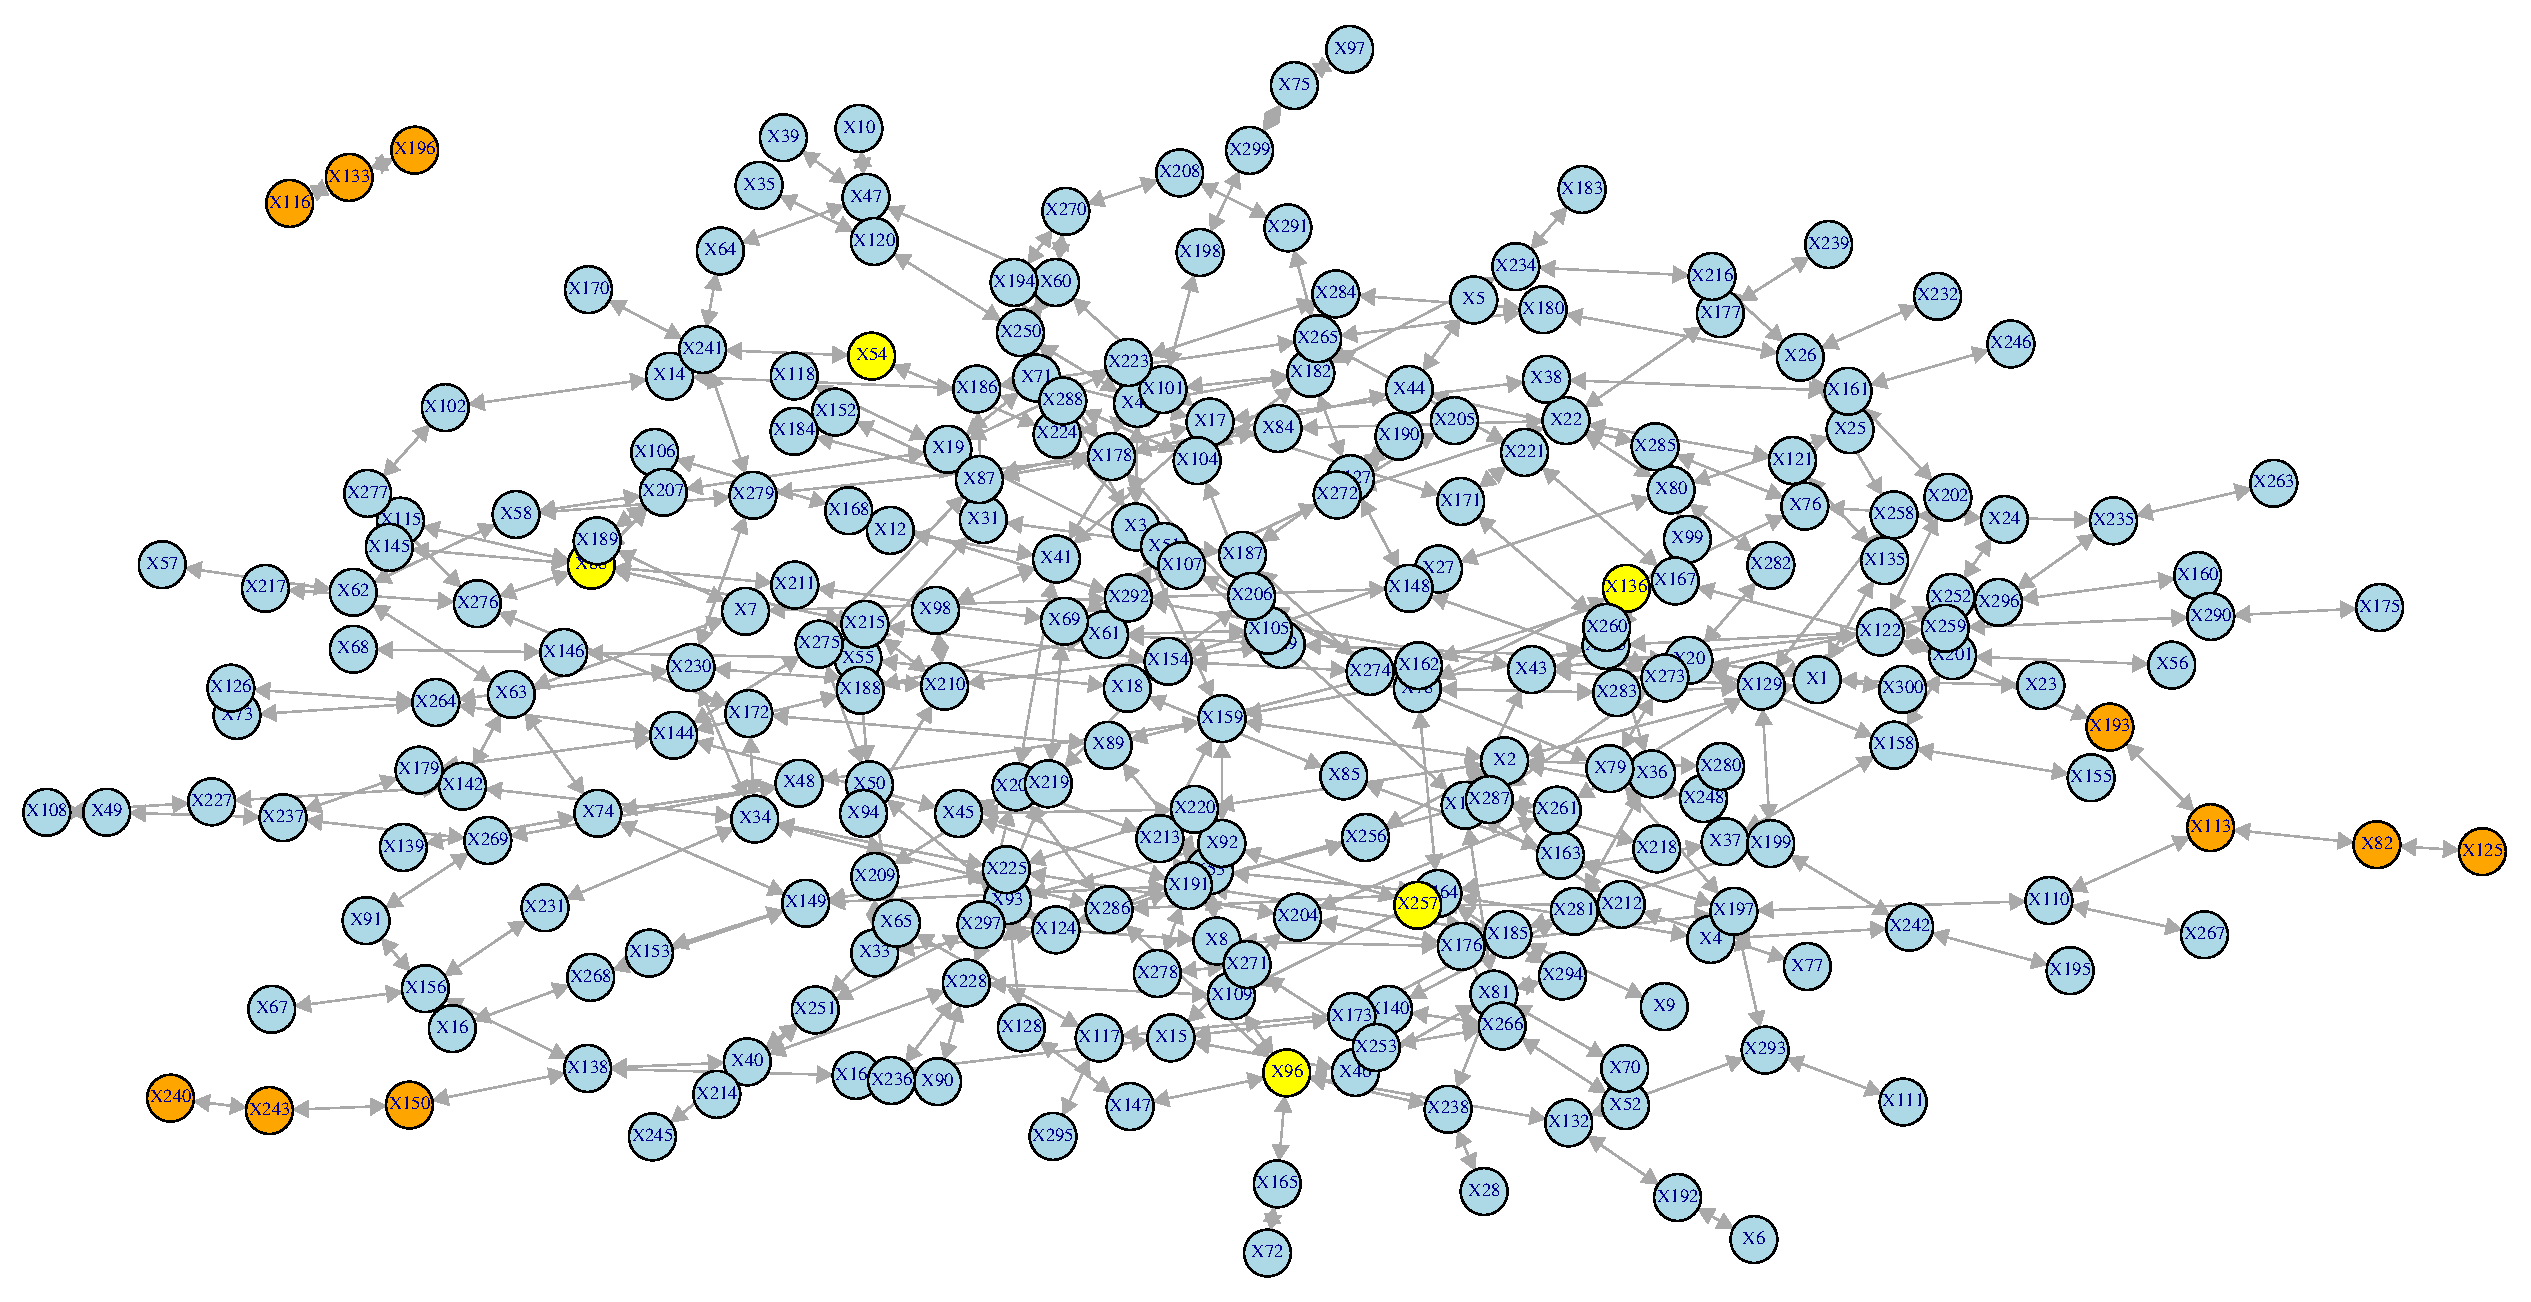
\includegraphics[width=\textwidth]{synthesized-easy}
          \caption{\tiny Easy}
        \end{figure}
        \begin{columns}
          \begin{column}{0.5\textwidth}
            \center
            \tiny
            \begin{tabular}{| c c || c c |}
              \hline
              \toprule
              \multicolumn{4}{c}{Original} \\ 
              \midrule \hline
              \boz X196   &  \boz X196  &
              X53   &  X53  \\ \hline
              X233   &  X233   &
              X39   &  X39  \\ \hline
              \ghool X88   &  \ghool X88  &
              \boz X196   &  \boz X133  \\ \hline
              \boz X116   &  \boz X116  &
              X127   &  X127  \\ \hline
              X197   &  X197  &
              X127   &  X148  \\ \hline
              X148   &  X148  &
              \boz X150   &  \boz X150  \\ \hline
              X148   &  X273  &
              \boz X116   &  \boz X133  \\ \hline
              X160   &  X160  &
              \ghool X96   &  \ghool X96  \\ \hline
              X95   &  X95  &
              X273   &  X273  \\ \hline
              \ghool X88   &  X115  &
              X40   &  X40  \\ \hline
              X53   &  X8  &
              X53   &  X164  \\ \hline
              X195   &  X195  &
              X56   &  X56  \\ \hline
            \end{tabular}
          \end{column}
          \begin{column}{0.5\textwidth}
            \center
            \tiny
            \begin{tabular}{| c c || c c |}
              \hline
              \toprule
              \multicolumn{4}{c}{Transformed} \\ 
              \midrule \hline
              \boz X196   &  \boz X196  &
              X233   &  X233  \\ \hline
              \boz X196   &  \boz X133  &
              \boz X133   &  \boz X133  \\ \hline
              \boz X133   &  \boz X116  &
              \boz X116   &  \boz X116  \\ \hline
              X95   &  X95  &
              \boz X240   &  \boz X240  \\ \hline
              X39   &  X39  &
              \boz X240   &  \boz X243  \\ \hline
              X59   &  X59  &
              X106   &  X106  \\ \hline
              \boz X243   &  \boz X243  &
              X106   &  X168  \\ \hline
              X114   &  X114  &
              X168   &  X168  \\ \hline
              \boz X243   &  \boz X150  &
              X56   &  X56  \\ \hline
              X39   &  X47  &
              X298   &  X298  \\ \hline
              \boz X150   &  \boz X150  &
              X247   &  X247  \\ \hline
              \boz X125   &  \boz X125  &
              X83   &  X83  \\ \hline
            \end{tabular}
          \end{column}
        \end{columns}
        \center{\tiny
        \begin{tabular}{| c c |}
          \hline
          AUC (Original): & 60.6 \\ 
          AUC (Transformed): & 62.4 \\
          wc p-value (paired): & 5.669e-09 \\ \hline
        \end{tabular}
        }
      \end{column}

      \begin{column}{0.3\textwidth}
        %\frametitle{Synthesized Data Medium Scenario}
        \begin{figure}
          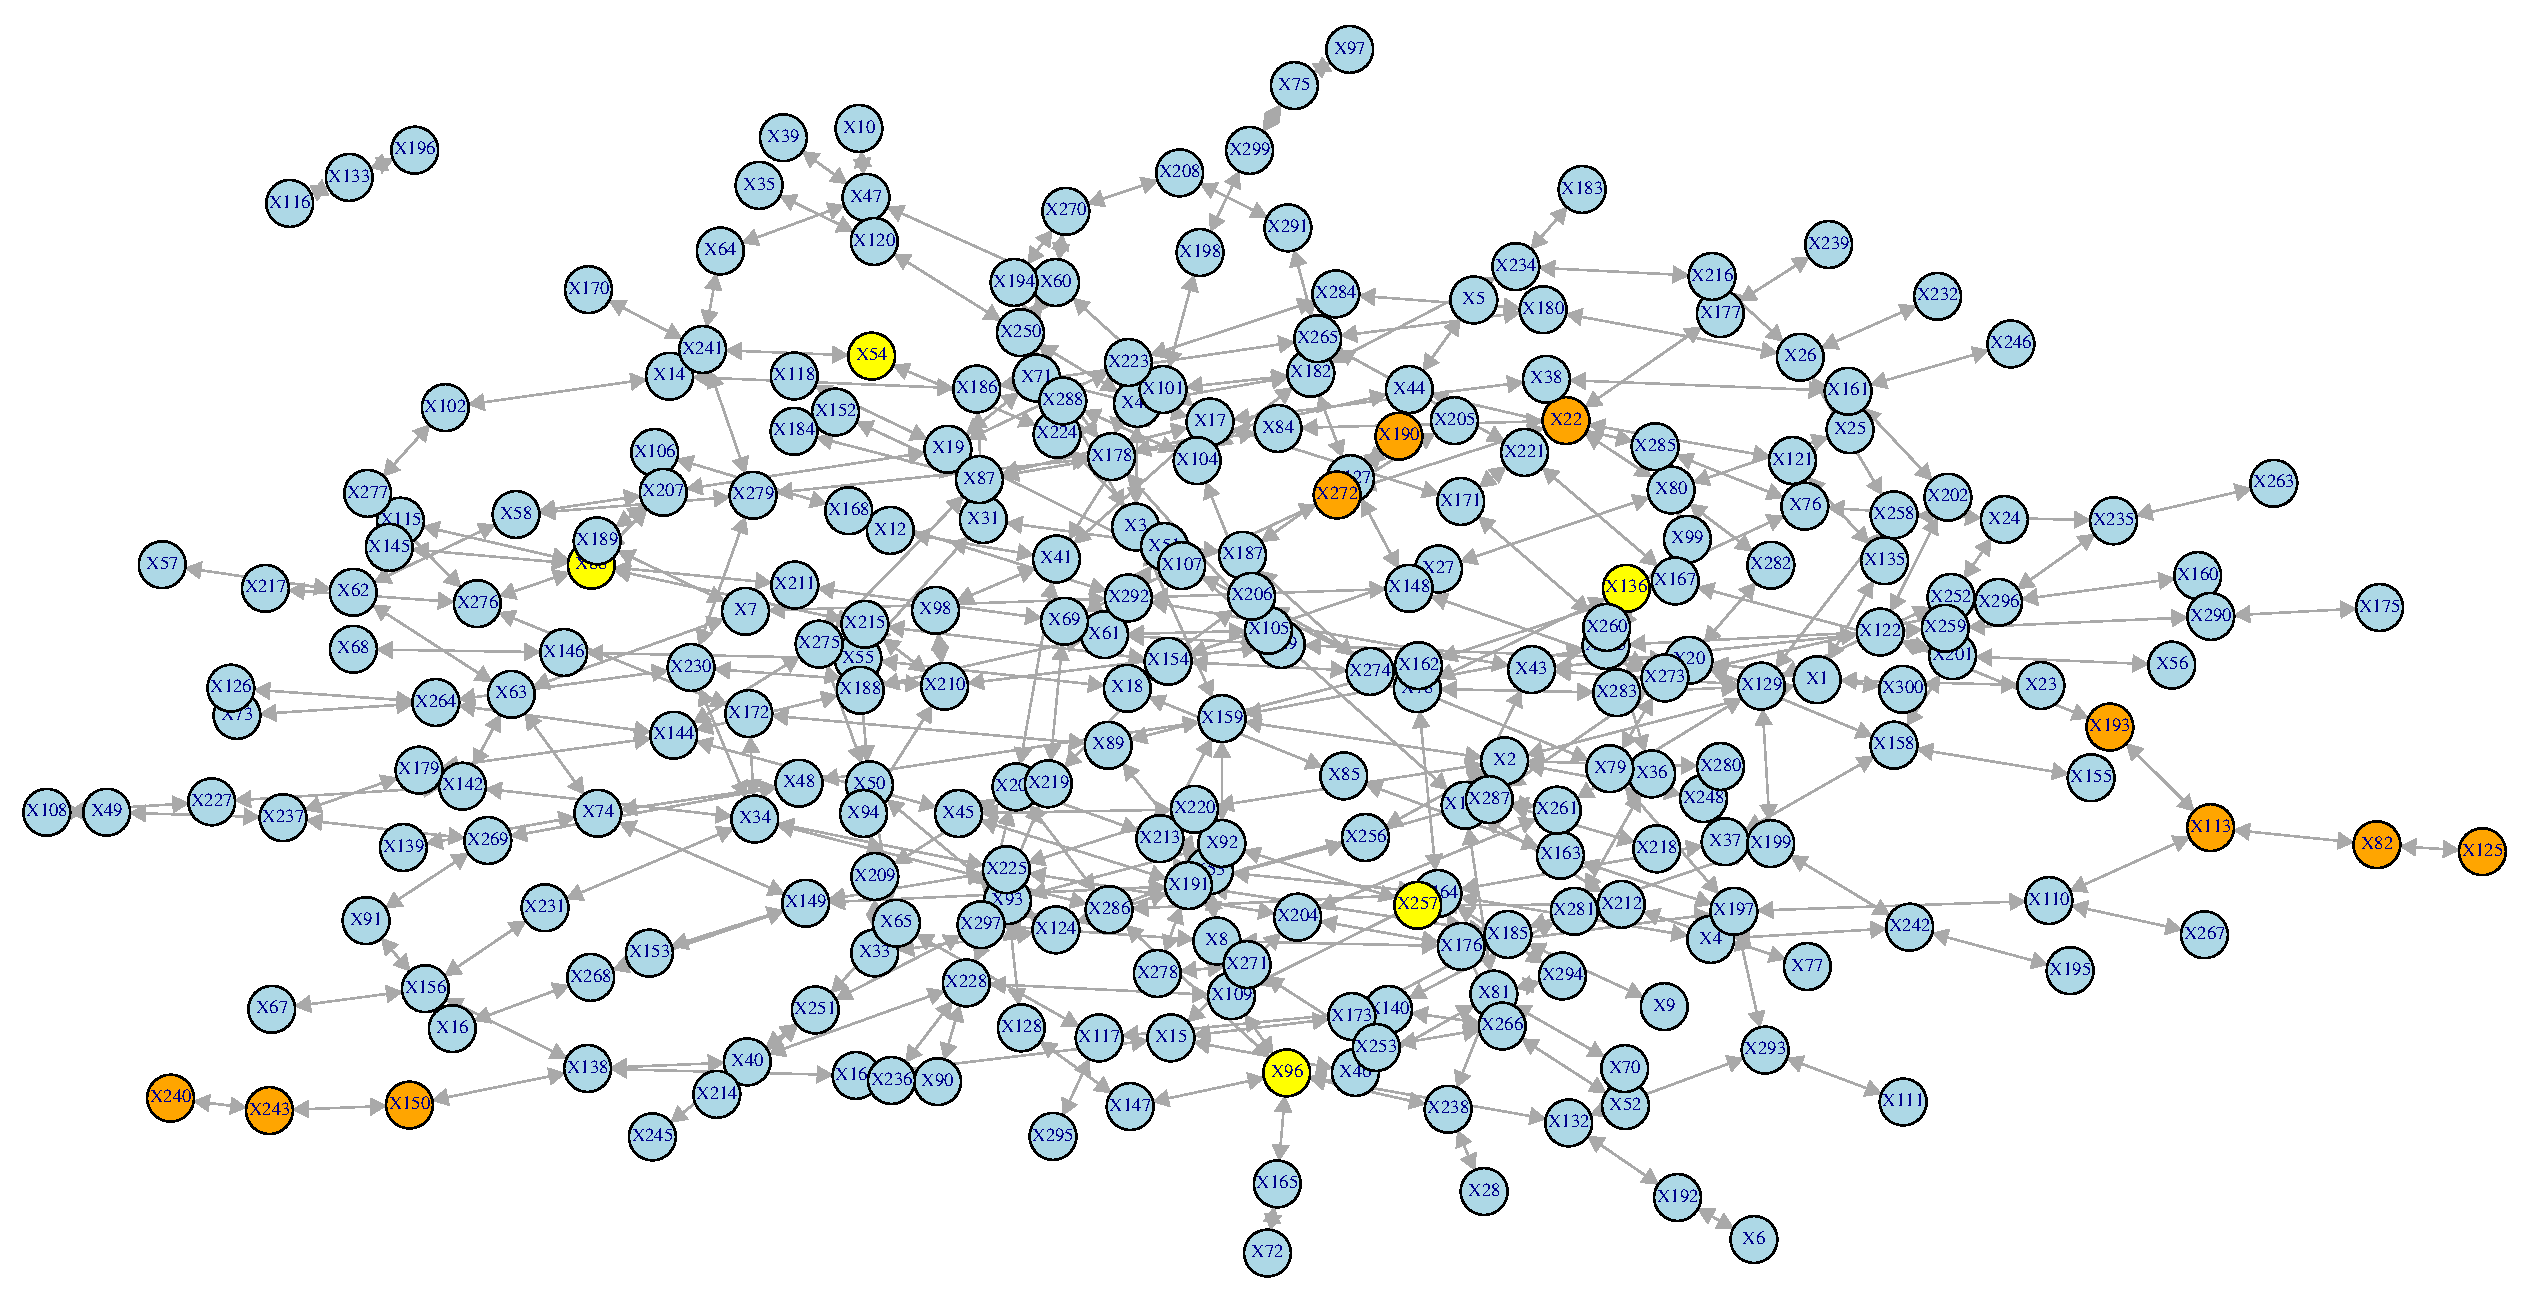
\includegraphics[width=\textwidth]{synthesized-medium}
          \caption{\tiny Medium}
        \end{figure}
        \begin{columns}
          \begin{column}{0.5\textwidth}
            \center
            \tiny
            \begin{tabular}{| c c || c c |}
              \hline
              \toprule
              \multicolumn{4}{c}{Original} \\ 
              \midrule \hline
              \boz X190   &  \boz X190 &
              X104   &  X104  \\ \hline
              X233   &  X233  &
              \boz X190   &  \boz X272  \\ \hline
              X277   &  X277  &
              \ghool X88   &  \ghool X88  \\ \hline
              \boz X190   &  X127  &
              X165   &  X165  \\ \hline
              \boz X272   &  \boz X272 &
              \boz X272   &  \boz X22  \\ \hline
              X106   &  X106  &
              X165   &  \ghool X96  \\ \hline
              \boz X150   &  \boz X150  &
              X250   &  X250  \\ \hline
              \ghool X88   &  X215  &
              \boz X22   &  \boz X22  \\ \hline
              X51   &  X51  &
              X28   &  X28  \\ \hline
              X73   &  X73  &
              X35   &  X35  \\ \hline
              X162   &  X162  &
              \boz X113   &  \boz X113  \\ \hline
              X112   &  X112  &
              X277   &  X102  \\ \hline
            \end{tabular}
          \end{column}
          \begin{column}{0.5\textwidth}
            \center
            \tiny
            \begin{tabular}{| c c || c c |}
              \hline
              \toprule
              \multicolumn{4}{c}{Transformed} \\ 
              \midrule \hline
              X233   &  X233  &
              \boz X190   &  \boz X190  \\ \hline
              X112   &  X112  &
              \boz X240   &  \boz X240  \\ \hline
              \boz X190   &  \boz X272 &
              \boz X240   &  \boz X243  \\ \hline
              X86   &  X86  &
              \boz X243   &  \boz X243  \\ \hline
              \boz X243   &  \boz X150 &
              \boz X190   &  X127  \\ \hline
              \boz X150   &  \boz X150  &
              \boz X272   &  \boz X272  \\ \hline
              X246   &  X246  &
              X298   &  X298  \\ \hline
              X106   &  X106  &
              \boz X125   &  \boz X125  \\ \hline
              X35   &  X35  &
              \boz X125   &  \boz X82  \\ \hline
              X247   &  X247  &
              \boz X272   &  X69  \\ \hline
              \boz X272   &  \boz X22 &
              \boz X82   &  \boz X82  \\ \hline
              X100   &  X100  &
              \ghool X257   &  \ghool X257  \\ \hline
            \end{tabular}
          \end{column}
        \end{columns}
        \center{\tiny
        \begin{tabular}{| c c |}
          \hline
          AUC (Original): & 60.1 \\ 
          AUC (Transformed): & 61.5 \\ 
          wc p-value (paired): & 1.383e-06 \\ \hline
        \end{tabular}
        }
      \end{column}

      \begin{column}{0.3\textwidth}
        \begin{figure}
          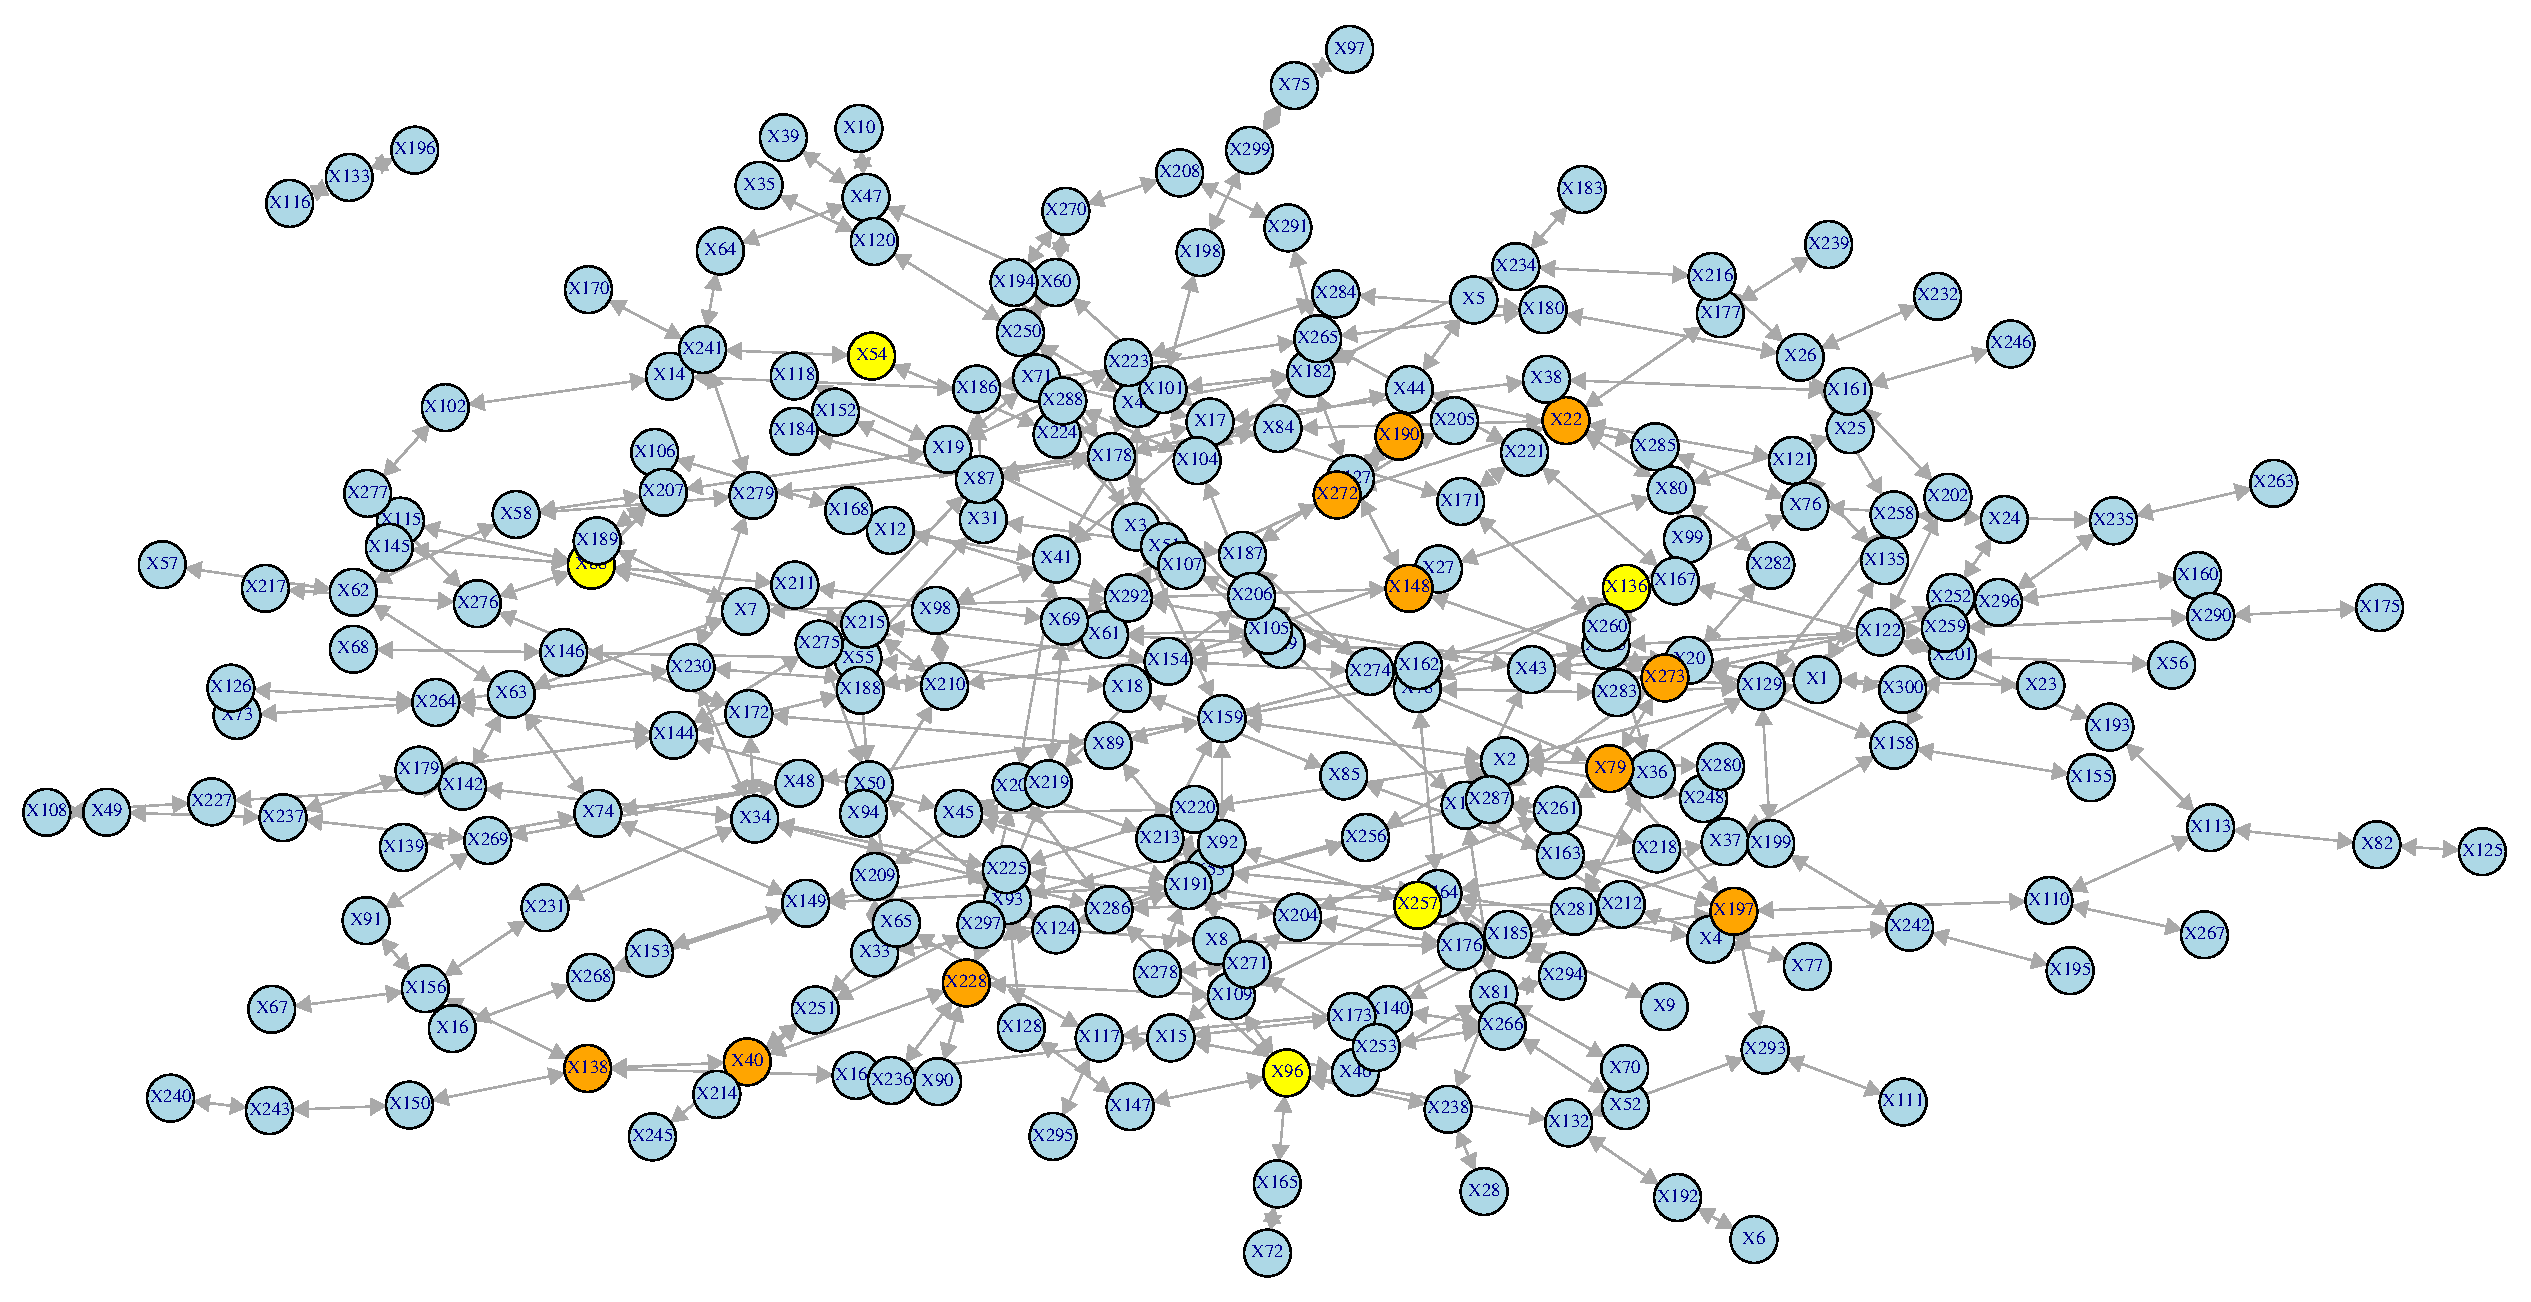
\includegraphics[width=\textwidth]{synthesized-hard}
          \caption{\tiny Hard}
        \end{figure}
        \begin{columns}
          \begin{column}{0.5\textwidth}
            \center
            \tiny
            \begin{tabular}{| c c || c c |}
              \hline
              \toprule
              \multicolumn{4}{c}{Original} \\ 
              \midrule \hline
              \boz X190   &  \boz X190  &
              X101   &  X101  \\ \hline
              X233   &  X233  &
              \boz X190   &  \boz X272  \\ \hline
              \ghool X88   &  \ghool X88  &
              X297   &  X297  \\ \hline
              \boz X190   &  X127  &
              X93   &  X93  \\ \hline
              X26   &  X26  &
              \boz X138   &  \boz X138  \\ \hline
              \boz X272   &  \boz X272 &
              \boz X272   &  \boz X22  \\ \hline
              X101   &  X41  &
              X123   &  X123  \\ \hline
              \boz X22   &  \boz X22 &
              X101   &  X198  \\ \hline
              X146   &  X146  &
              \boz X228   &  \boz X228  \\ \hline
              X278   &  X278  &
              X72   &  X72  \\ \hline
              \ghool X88   &  X115 &
              \ghool X96   &  \ghool X96  \\ \hline
              \boz X148   &  \boz X148 &
              X112   &  X112  \\ \hline
            \end{tabular}
          \end{column}
          \begin{column}{0.5\textwidth}
            \center
            \tiny
            \begin{tabular}{| c c || c c |}
              \hline
              \toprule
              \multicolumn{4}{c}{Transformed} \\ 
              \midrule \hline
              X233   &  X233  &
              \boz X190   &  \boz X190  \\ \hline
              X112   &  X112  &
              \boz X190   &  \boz X272  \\ \hline
              X86   &  X86  &
              \boz X190   &  X127  \\ \hline
              \boz X272   &  \boz X272 &
              \boz X272   &  X205  \\ \hline
              X205   &  X205  &
              X146   &  X146  \\ \hline
              X146   &  X68  &
              X68   &  X68  \\ \hline
              X298   &  X298  &
              \boz X272   &  \boz X22  \\ \hline
              X90   &  X90  &
              X127   &  X127  \\ \hline
              X100   &  X100  &
              \boz X272   &  X69  \\ \hline
              X297   &  X297  &
              X72   &  X72  \\ \hline
              X127   &  \boz X148 &
              X155   &  X155  \\ \hline
              X247   &  X247  &
              X196   &  X196  \\ \hline
            \end{tabular}
          \end{column}
        \end{columns}
        \center{\tiny
        \begin{tabular}{| c c |}
          \hline
          AUC (Original): & 60.2 \\ 
          AUC (Transformed): & 62.5 \\ 
          wc p-value (paired): & 8.151e-13 \\ \hline
        \end{tabular}
        }
      \end{column}

    \end{columns}

    \vspace{1cm}
      \mytitle{References and Acknowledgment}
    \begin{columns}[T]
%      \left
      \begin{column}{0.8\textwidth}
        \tiny
        Acknowledgment:\\
        Prof. Dr. Dr. Thomas Lengauer, Sarvesh Nikumbh, Nora Speicher, Anna Feldmann.\\
        References:\\
        1. van't Veer, Laura J., et al. "Gene expression profiling predicts clinical outcome of breast cancer." nature 415.6871 (2002): 530-536.\\
        2. Barab�si, Albert-L�szl�, and Zoltan N. Oltvai. "Network biology: understanding the cell's functional organization." Nature Reviews Genetics 5.2 (2004): 101-113.\\
        3. Lavi, Ofer, Gideon Dror, and Ron Shamir. "Network-induced classification kernels for gene expression profile analysis." Journal of Computational Biology 19.6 (2012): 694-709.\\
      \end{column}
    \end{columns}
  \end{frame}
\end{document}

